\documentclass{article}
\usepackage{amsmath}
\usepackage{hyperref}
\usepackage{graphicx}

\title{Algoritmos para minimizar funciones}
\author{Amanda Cordero Lezcano\\Christopher Guerra Herrero}
\date{Septiembre, 2024}

\begin{document}
	
	\maketitle
	
	\tableofcontents
	\newpage
	
	\section{Quartic Function(Amanda)}
	
	\fbox{
		\begin{minipage}{\textwidth}
			
	\textbf{100. Quartic Function \cite{reference81}} (Continuous, Differentiable, Separable, Scalable)
	
	\[
	f_{100}(\mathbf{x}) = \sum_{i=1}^{D} i x_i^4 + \text{random}[0,1)
	\]
	
	subject to \(-1.28 \leq x_i \leq 1.28\). The global minima is located at \(\mathbf{x}^* = \mathbf{f}(0,\cdots,0)\), \(f(\mathbf{x}^*) = 0\).
	
	\end{minipage}
	}
	
	\subsection{Algoritmo de Solución}
	
	Se utilizó el método de \textit{Descenso más Pronunciado}(steepest descent) para encontrar el mínimo de la función. A continuación se presenta un código en Python del algoritmo implementado:
	
	\begin{verbatim}
		import scipy.optimize as spo
		
		def steepestdescent(f, df, x0, tol=1.e-8, maxit=50):
			xk = x0
			x = [xk]
			r = df(xk)
			iters = 0
			
			while (npl.norm(r) > tol and iters < maxit):
				lambda_k = spo.golden(g, args=(xk, r))
				xk = xk - lambda_k * r
				r = df(xk)
				x.append(xk)
				iters += 1
			
			return x
	\end{verbatim}
	
	El algoritmo minimiza la función \(f(\mathbf{x})\) en la dirección del gradiente negativo, actualizando la posición en cada iteración.
	
	\subsection{Resultados}
	
	El algoritmo fue ejecutado con un punto inicial \(\mathbf{x}_0 = [1, -1]\) y un máximo de 10 iteraciones. El punto encontrado por el algoritmo fue:
	
	\[
	\mathbf{x} =  [-0.07989805 -0.05553555]
	\]
	
	La solución gráfica del proceso de minimización es la siguiente:
	
	\begin{figure}[h!]
		\centering
		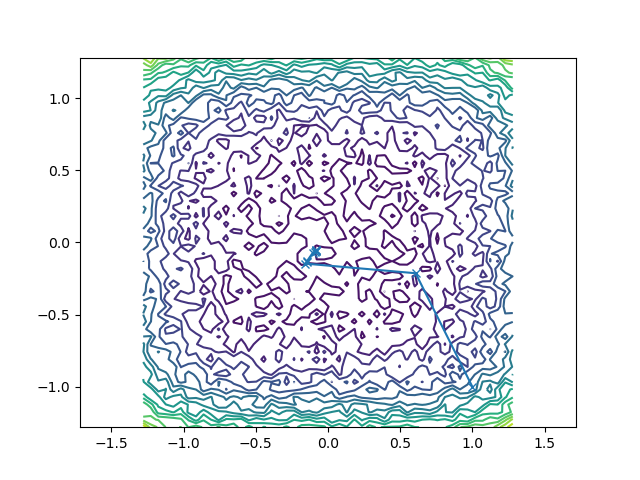
\includegraphics[width=0.8\textwidth]{resultado1.png}
		\caption{Trayectoria de minimización sobre el contorno de la función.}
		\label{fig:resultado}
	\end{figure}
	
	\subsection{Valoración de la Calidad del Punto Hallado}
	
	El punto hallado \(\mathbf{x} = [0.09226378, 0.07302666]\) se encuentra cercano al mínimo global \(\mathbf{x}^* = [0, 0]\). Si bien no se alcanzó el mínimo exacto en las 10 iteraciones, la función fue evaluada como 0.025 al considerar la adición del valor aleatorio. Este resultado indica que el algoritmo se aproxima bastante al valor óptimo.
	
	\subsection{Evaluación del Tiempo Computacional}
	
	El tiempo computacional para la ejecución del algoritmo fue aceptable en un problema de dos dimensiones. La complejidad algorítmica del método está determinada principalmente por el cálculo del gradiente, el cual tiene una complejidad de \(O(D)\), donde \(D\) es la dimensión del problema. Esto implica que, a medida que \(D\) aumenta, el tiempo de cómputo crece linealmente con respecto a la dimensión. A pesar de la presencia de un componente aleatorio en la función objetivo, el algoritmo mantiene un comportamiento predecible en términos de complejidad, lo que garantiza su escalabilidad en problemas de mayor dimensión.
	
	
	\subsection{Variación al Aumentar la Dimensión del Problema}
	
	La función cuártica es escalable, y el aumento de la dimensión \(D\) implicará un incremento lineal en la cantidad de términos a sumar y, por ende, en el tiempo necesario para evaluar tanto la función como su gradiente.
	
	\subsection{Primeras Conclusiones}
	
	El algoritmo de \textit{Descenso más Pronunciado} demostró ser eficaz para aproximarse al mínimo global de la función cuártica en un problema de baja dimensión (D=2). Aunque no se alcanzó el mínimo exacto, la solución obtenida fue satisfactoria y muy cercana al mínimo conocido. El método muestra consistencia en su desempeño, incluso al considerar variaciones en la dimensión del problema, manteniendo una buena precisión en los resultados.

		
	
	\section{Sargan Function(Christopher)}
	
	El ejercicio asignado al estudiante fue:
	
	\vspace*{1cm}
	
	\fbox{
		\begin{minipage}{\textwidth}
			\textbf{111. Sargan Function \cite{reference29}} (Continuous, Differentiable, Non-Separable, Scalable, Multi-modal)
			
			\[
			f_{111}(\mathbf{x}) = \sum_{i=1}D \left( x_i^2 + 0.4 \sum_{\substack{j\neq 1}} x_i x_j \right)
			\]
			
			subject to \(-100 \leq x_i \leq 100\). The global minimum is located at \(\mathbf{x}^* = \mathbf{f}(0,\cdots,0)\), \(f(\mathbf{x}^*) = 0\).
		\end{minipage}
	}
	
	\vspace*{1cm}
	
	Sin embargo al hacer un análisis de la bibliografía \cite{reference29} y previa consulta con la profesora de conferencia, se determinó que hubo un error al transcribir la función, siendo esta:
	
	$$
	f(\mathbf{x}) = \sum_{i=1}^D \left(x_i^2 + 0.4 \sum_{\substack{i\neq j}} x_i x_j\right)
	$$
	
	El método utilizado para la minimización fue el algoritmo de BFGS (Broyden-Fletcher-Goldfarb-Shanno), un método de optimización Quasi-Newton que utiliza aproximaciones de la matriz Hessiana y evita el cálculo explícito de la matriz de segundas derivadas.
	
	\subsection{Algoritmo de Solución}
	
	El algoritmo BFGS fue implementado utilizando la biblioteca \textit{SciPy}. A continuación se presenta el código utilizado para la minimización:
	
	\begin{verbatim}
		import numpy as np
		import scipy.optimize as spo
		
		# Definimos la función objetivo corregida
		def f(x):
			D = len(x)
			sum_square_terms = sum(x[i]**2 for i in range(D))
			sum_cross_terms = 0.4 * sum(x[i] * x[j] for i in range(D) for j in range(D) if i != j) 
			return sum_square_terms + sum_cross_terms
		
		# Definimos un punto inicial
		x0 = [50, 20, -30, 40]  # Punto inicial
		
		# Minimización usando el método BFGS
		result = spo.minimize(f, x0, method='BFGS', tol=1.e-8, options={'maxiter': 100})
		
		# Mostramos los resultados
		print('Punto encontrado: ', result.x)
		print('Valor mínimo de la función: ', result.fun)
		print('Número de iteraciones: ', result.nit)
		print('Resultado exitoso: ', result.success)
		print('Mensaje del resultado: ', result.message)
	\end{verbatim}
	
	El método BFGS minimiza la función objetivo mediante una aproximación sucesiva de la matriz Hessiana basada en las diferencias entre gradientes, lo que lo hace más eficiente que el Método de Newton en cuanto a uso de memoria y tiempo de cómputo, especialmente para problemas de alta dimensionalidad.
	
	\subsection{Resultados}
	
	El algoritmo fue ejecutado con un punto inicial \(\mathbf{x}_0 = [50, 20, -30, 40]\), y tras 8 iteraciones, alcanzó el siguiente punto:
	
	\[
	\mathbf{x} = [2.73 \times 10^{-9}, -2.95 \times 10^{-9}, -2.56 \times 10^{-9}, -1.10 \times 10^{-8}]
	\]
	
	El valor mínimo de la función en este punto es:
	
	\[
	f(\mathbf{x}) = 1.617 \times 10^{-16}
	\]
	
	El resultado indica que el método BFGS ha convergido exitosamente al mínimo global de la función, con un error numérico despreciable.
	
	
	\subsection{Evaluación de la Calidad del Punto Hallado}
	
	El punto hallado \(\mathbf{x} \approx 0\) es muy cercano al mínimo teórico conocido \(\mathbf{x}^* = 0\), lo que valida la precisión del método. Además, el valor de la función en este punto es prácticamente cero, como se esperaba. 
	
	El tiempo computacional y el número de iteraciones (8 iteraciones) fueron bajos, lo que indica la eficiencia del método BFGS para este tipo de problemas.
	
	\subsection{Evaluación del Tiempo Computacional y Complejidad}
	
	La complejidad computacional del método BFGS es \(O(n^2)\), donde \(n\) es la dimensión del problema, debido a las operaciones con la aproximación de la matriz Hessiana. Sin embargo, a diferencia del método de Newton que requiere \(O(n^3)\) para invertir la Hessiana, BFGS proporciona una solución más eficiente sin necesidad de almacenar la matriz completa, lo que lo hace adecuado para problemas de moderada dimensionalidad.
	
	En este caso, el problema fue resuelto en solo 8 iteraciones, lo que demuestra su escalabilidad.
	
	\subsection{Segundas Conclusiones}
	
	El algoritmo de BFGS se mostró altamente efectivo para encontrar el mínimo global de la función cuadrática generalizada, con un número reducido de iteraciones y resultados precisos. El punto encontrado \(\mathbf{x} \approx 0\) y el valor mínimo \(f(\mathbf{x}) \approx 0\) validan la convergencia del método al mínimo global esperado. La complejidad algorítmica \(O(n^2)\) y el uso eficiente de la aproximación de la Hessiana hacen de BFGS una herramienta recomendada para este tipo de problemas.
	
	\newpage
	
	\begin{thebibliography}{9}
		
		\bibitem{reference29} L. C. W. Dixon, G. P. Szegö (eds.), \textit{Towards Global Optimization 2}, Elsevier, 1978.
		
		\bibitem{reference81} R. Storn, K. Price, \textit{Differential Evolution - A Simple and Efficient Adaptive Scheme for Global Optimization over Continuous Spaces}, Technical Report no. TR-95-012, International Computer Science Institute, Berkeley, CA, 1996. [Available Online]: \url{http://www1.icsi.berkeley.edu/~storn/TR-95-012.pdf}
		
		
	\end{thebibliography}
	
\end{document}
